\subsection{Rising Waves: The Cheerful Dance of Antenna Patterns!}

\begin{tcolorbox}[colback=gray!10, colframe=black, title=E9C13]  
How does the radiation pattern of a horizontally polarized antenna vary with increasing height above ground?

\begin{enumerate}[label=\Alph*]
    \item The takeoff angle of the lowest elevation lobe increases
    \item \textbf{The takeoff angle of the lowest elevation lobe decreases}
    \item The horizontal beamwidth increases
    \item The horizontal beamwidth decreases
\end{enumerate} \end{tcolorbox}

\subsubsection{Related Concepts}

The behavior of a horizontally polarized antenna as its height above the ground increases is an essential concept in radio communication. The radiation pattern of the antenna is largely influenced by its height relative to the ground, which can affect the signals transmitted and received.

The takeoff angle is defined as the angle at which the majority of the energy is radiated away from the antenna into space. For antennas situated close to the ground, such as dipole antennas, the radiation pattern will show a higher takeoff angle. However, as the height of the antenna increases, the takeoff angle will decrease. This phenomenon can be attributed to the improved clearance of ground effects, which allows the radio waves to propagate more freely.

\subsubsection{Calculation Steps}

To understand this concept mathematically, consider a scenario where the height \(h\) of the antenna above ground increases. The effective gain of the antenna can be correlated to its height. As the antenna rises:

1. The effective radius of the ground wave increases.
2. The takeoff angle can be approximated using the formula:

\[
\theta = \tan^{-1}\left(\frac{h}{d}\right)
\]

where \( \theta \) is the takeoff angle, \( h \) is the height of the antenna, and \( d \) is the distance from the antenna to the horizon.

As \(h\) increases, the distance \(d\) also increases, resulting in a reduction of the slope (and hence the angle \(\theta\)).

\subsubsection{Diagram}

The following diagram illustrates the relationship between the height of the antenna and the takeoff angle. 

\begin{center}
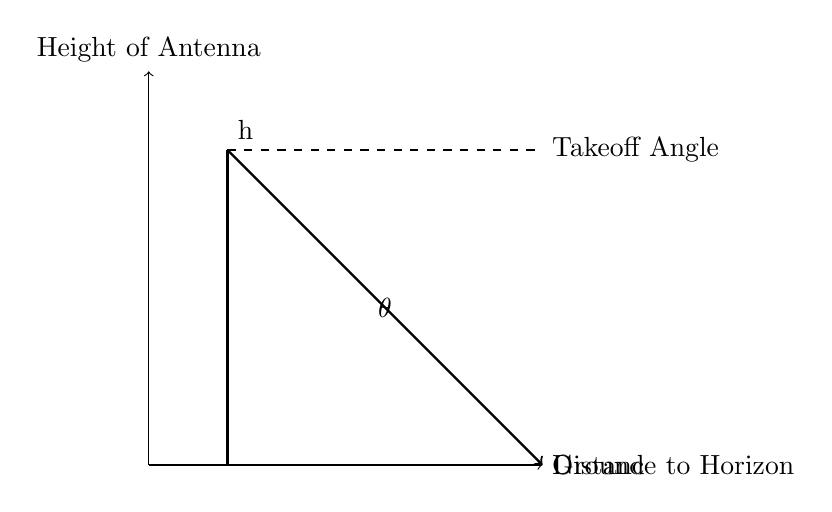
\begin{tikzpicture}
    \draw[->] (0,0) -- (5,0) node[right] {Distance to Horizon};
    \draw[->] (0,0) -- (0,5) node[above] {Height of Antenna};

    \draw[thick] (1,0) -- (1,4) node[above right] {h};

    \draw[dashed] (1,0) -- (5,0) node[right] {Ground};
    \draw[dashed] (1,4) -- (5,4) node[right] {Takeoff Angle};

    \draw[thick, ->] (1,4) -- (5,0);

    \node at (3,2) {\(\theta\)};
\end{tikzpicture}
\end{center}

As depicted in the diagram, increasing the height \(h\) leads to a decrease in the takeoff angle \(\theta\). Therefore, the correct answer to the question is that the takeoff angle of the lowest elevation lobe decreases as the height of a horizontally polarized antenna increases above ground.